\documentclass{article}
\usepackage{amsmath}
\usepackage{amssymb}
\usepackage{graphicx}
\usepackage{enumitem}
\usepackage[utf8]{inputenc}
\graphicspath{{/home/stephanie/Escritorio/THC/Taller-de-Herramientas-Computacionales/Clases/Latex/Imagenes/}}

\title{\Huge Taller de Herramientas Computacionales}
\author{Stephanie Escobar Sánchez}
\date{17/enero/2019}
\begin{document}
	\maketitle
\begin{center}
	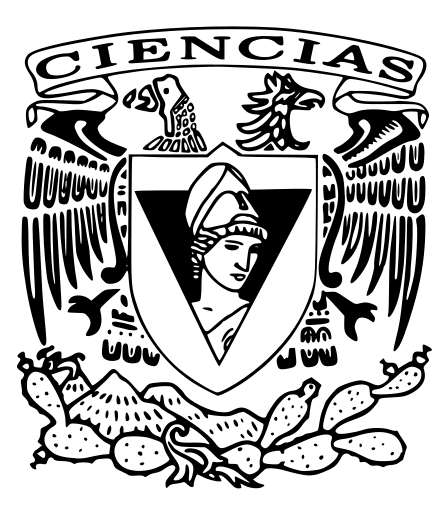
\includegraphics[scale=0.40]{1.png}	
\end{center}
\newpage
\title{\Huge Bitácora clase 9} \\
\\
Comenzamos viendo cómo hacer un libro en LaTeX, comenzando por poner \textit{documentclass{book}} para que nos cree un documento con el formato de libro, y para que las secciones aparezcan en español utilizamos la biblioteca babel, que en un principio no se podía descargar, utilizamos synaptic en ubunto, que es un gestor de paquetes y nos permitio descargar los paquetes faltantes.\\
\\
Como el formato es un libro utilizamos chapter{} para crear capítulos dentro de él y utilizamos section{} para crear secciones, con tableofcontens te crea un índice donde automáticamente agrega las secciones. El paquete hyperref te permite agregar links de páginas directo al documento. Y el comando verbatim te permite agregar código sin cambiar el formato. Además hay paquetes que te permiten agregar bibliografía y acomodarla en la sección final, con el nombre del autor y el título del libro. Otra cosa importante es saber que hay paquetes en LaTeX y que todo está documentado en la web por lo que si queremos saber cómo funciona algo o cómo hacer una función en específico. \\
\\
Después de ver LaTeX, solucionamos un problema de la tarea, teníamos que hacer una función que nos diera el máximo común divisor de una pareja de números. Para comenzar a resolver el problema lo más importante fue entenderlo, por lo que lo primero que hicimos fue pensar en una solución a mano, utilizamos el algoritmo de Euclides, que ve a todo número natural como (p*q)+r y a partir de eso fuimos haciendo más cálculos en el pizarrón a modo de acomodarlo de la forma más conveniente sin hacerle nada. Con el comando \% es posible obtener el residuo de una división y fue lo que hicimos. Con eso solucionamos el problema, primero a mano y después en el programa. Es por ello que es importante primero pensar en una solución sin pensar en el código y después ver qué funciones necesitas para llegar al resultado. Otra cosa importante es siempre pensar en la solución más sencilla y que tenga menos lineas para no confundirnos, se  tiene que reflexionar si es la forma más corta o hay una mejor.\\
\\
Al final de la clase tuvimos problemas para importar archivos desde una carpeta, el problema fue que el directorio que estaba en la terminal desde donde abrimos el idle era diferente al directorio donde estaba guardado el programa que queríamos abrir. Para ello, con el comando cd es posible cambiar de directorios directamente en el idle para poder buscar los archivos que necesitamos. 


\end{document}